\section{CLI}

\begin{figure}
\centering
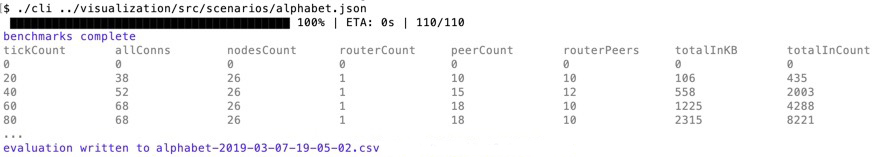
\includegraphics[width=1\textwidth]{graphics/analysis-tools/cli.jpg}
\caption{CLI}
\label{fig:anl-cli}
\end{figure}

As the visualisation is doing some heavy lifting to visualise the state of each node, it is not really suitable for large scenarios. Also, using it for benchmarking with different parameters is a tedious task. It is very good for analysing and debugging small scenarios, yet it has its limits for performance and scaling analysis.

Thus, a \glsfirst{cli} has been developed which runs the simulation in a headless mode in a Node.js environment. It accepts a path to a scenario JSON as paramter and also accepts a log level. By default the logging is turned off but can be turned on by the log level parameter. The scenario is executed and the results are printed (\vref{fig:anl-cli})and saved as a \gls{csv} file. A JSON file is exported with the current state of the nodes. The file can be imported into the visualisation to visually analyse the state.

Not only is it faster to run a scenario, it also accepts a new type of configuration in the scenario which allows benchmarking. The parameter allows running one scenario in a batch job with different settings for Mitosis. The parameter can be configured in the scenario. When the benchmark is finished the CLI also saves the results as a \gls{csv} and as a JSON file.
